

\section{Iterations}


\subsection {Testing mobile app technology, conceptual model}
The goal of this iteration was to make a prototype using the proposed technology. The prototype will tell us if it is sensible to use the technology for the project, as well as having a conceptual model to use when discussing initial ideas around the aim of the project, functionality, as well as interaction design.

The technology to be tested was React Native. The reason for this to be the first choice, was to support multiple platforms and not having to rewrite the application for every platform. The same application can be used for Android and iPhone with little modification to the code. React Native is build upon the React front end web development framework, which means some code can be reused for web as well. But all the the views need to be modified, as they use specific React Native components for mobile units. React and React Native are JavaScript frameworks.

We have also used the React web  development framework in previous projects. It s one of the more popular and mature front end web development frameworks in the market. 

The prototype itself and the development process showed that the technology could be used for displaying and organize CPGs. Lessons learned about content flow, databases, app navigation, displaying information and dialogues. JavaScript in the view gives a lot of flexibility compared to just tags.

\begin{figure}[h!]
	\caption {A very simple conceptual model to test one of the proposed technologies, as well as acting as a starting point for discussions}
	\label{fig:ConseptualModel}
	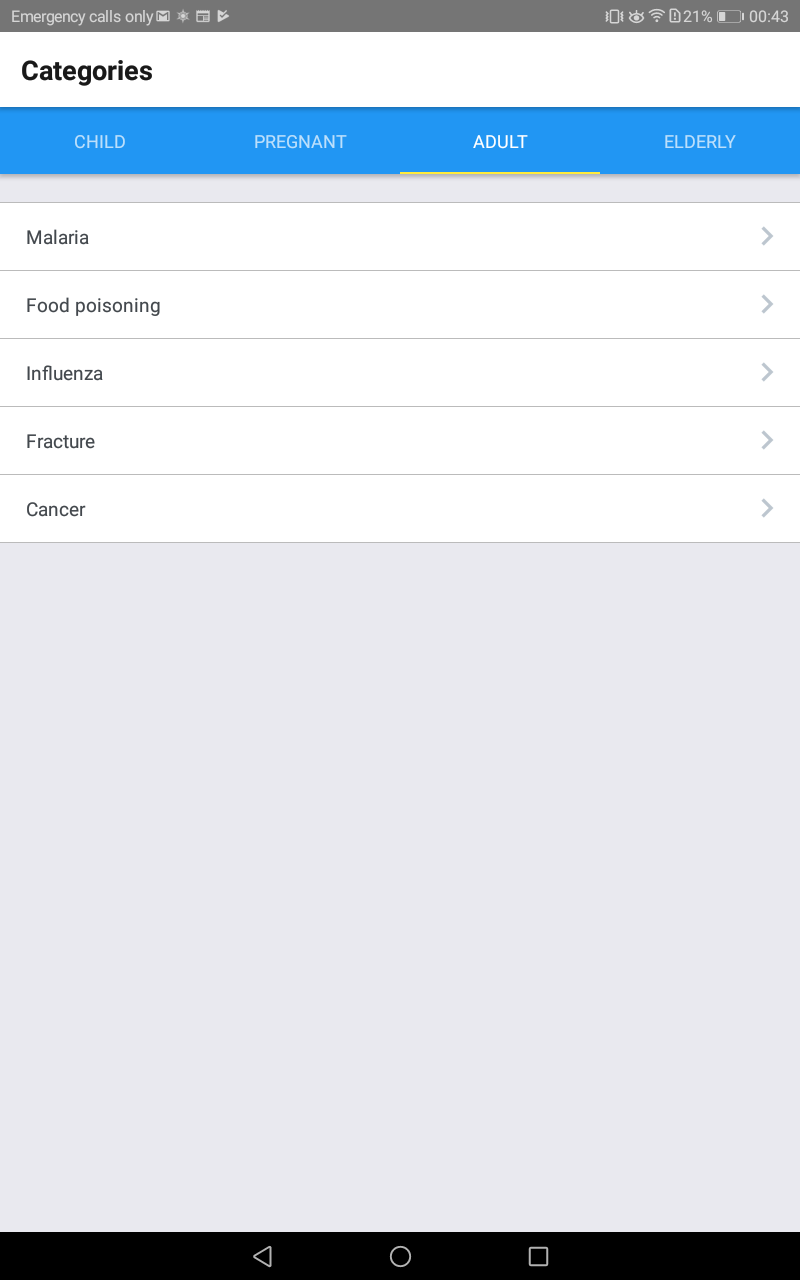
\includegraphics[scale=0.1]{ConceptualPrototype}
\end{figure}

The interface was evaluated with the supervisors, using cognitive walkthroughs. It also worked as a conceptual model, using the prototype as a base for discussing ideas. Both for discussing the purpose of the project, what the user should be able to do, how to organize content and what functionality to add.


\subsection{Studying similar products}
The purpose of the iteration is to see what exists in the market. What have others done. What can we improve, where can we add value to both the medical community and to computer science.

The results from this iteration is presented in appendix \ref{appendix:ComparisonApps}. As a conclusion, none of these application have a data model which can represent CPGs, nor a patient in a clinical encounter. The representations of CPGs are mostly text based, flow charts or flow charts which expand when you click on decision vertices. LIFE: Neonatal Resuscitation Training is a pretty advanced 3D game, but there is no data model representing the content in the quizzes and tasks.

\subsection{Technology used to represent CPGs}
In this iteration we evaluated technologies which could be used to model CPGs.

\begin{itemize}
	\item \textbf{GLIF}
	\item \textbf{Proforma}
	\item \textbf{Asbru}
	\item \textbf{DPF}
\end{itemize}



\subsection{Designing alternatives}

\subsection {Entity and workflow models}
The goal of the iteration was to model patients at different stages of the clinical encounter. The entity model should be able to represent patients in scenarios in quizzes with answer keys.

We based our models on the paediatric possible asthma guideline \cite{RepublicofKeny2016}. The first step was to understand every symptom, medication, equipment used in the treatment and keywords such as "admit". Resources like \textcite{Disease2011} and \textcite{Johansen2018} were some of the resources used, but most importantly was an expert of domain. 

The developer made a prototype of his understanding of the CPG, which simulated a clinical encounter with a patient. See figure \ref{fig:SimulationTool} The simulation would start with listing symptoms of asthma and the clinician would choose among the symptoms, redirecting to the treatment for severe, mild, moderate and no asthma. The simulation would continue with cycles of evaluating the given treatment, and the clinician needs to act accordingly to the evaluation for each cycle until the treatment can be ended. An expert of domain got the task of going through the entire simulations of use cases such as "a patient with severe asthma responds poorly to salbutamol treatment". The stimulation gave a thorough understanding of the guideline, emphasized details which would have been missed or details of the treatment which is left out of the guideline itself, such as differential diagnoses.

\begin{figure}[h!]
	\caption {Screenshots of the prototype used to simulate a clinical encounter with a domain expert}
	\label{fig:SimulationTool}
	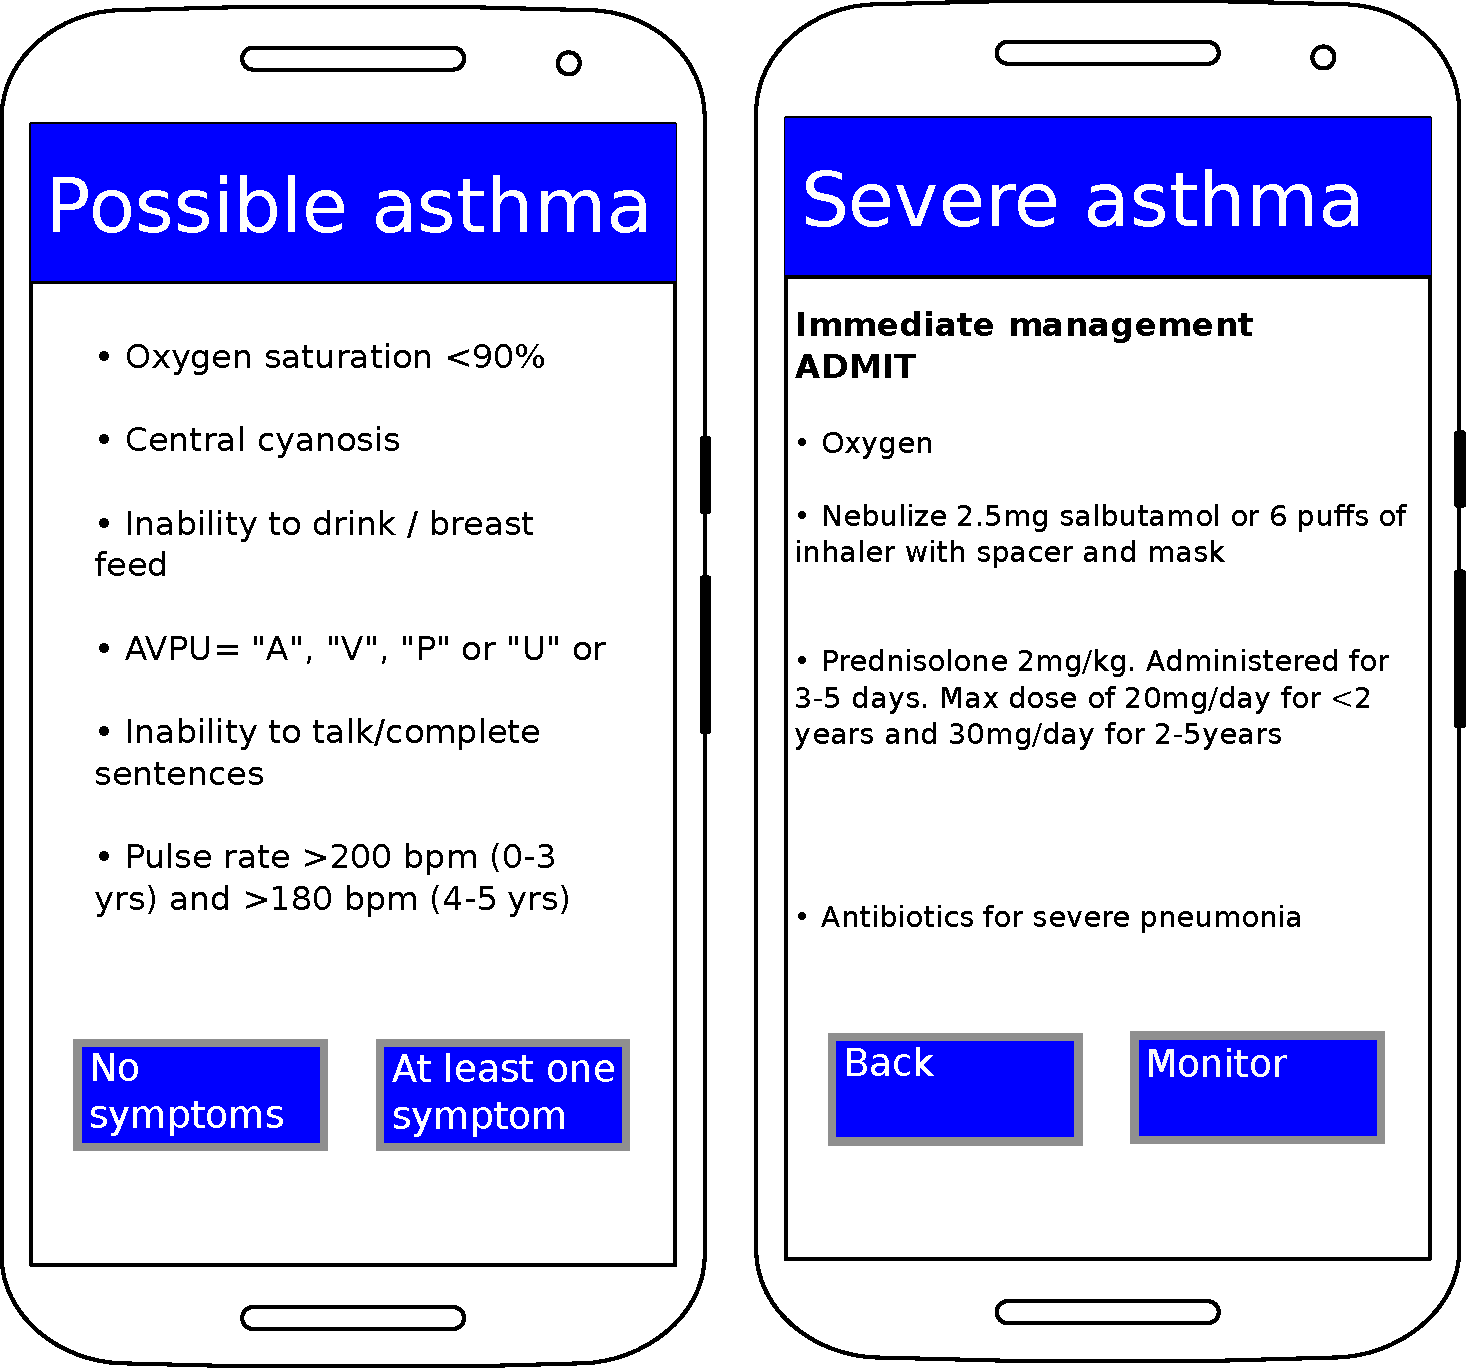
\includegraphics[scale=0.6]{SimulationTool}
\end{figure}

The guideline is also unclear at some points, where a discussion with a domain expert was needed. For example: wheeze + history of cough or difficulty breathing. When parentheses are not used, it is difficult to see if wheeze always needs to be  present, or if it is enough that cough alone is. It is also difficult to understand the effect and model the situation where the presence of a symptom at a certain age gives "increased likelihood" for asthma. In computer science the terms need to be very clear.

For evaluating the entity model, a domain expert made quizzes with factual questions as well as scenario based. By replacing patient related variables in the questions and scenarios, with tags pointing to variables in the entity model, we could see whether the model fulfilled the requirements of displaying good and valid sentences. The sentences were equally good and valid when using different instances of the entity model.

The workflow model got evaluated by making quiz scenarios, and by confirming that these scenarios covered the entire guideline.



 
\subsection{User interface}
\subsection{Game Engine}
\subsection{Content flow and creating questions}



\subsection{Focus group}

\subsection{Workshop}